%\documentclass[main.tex]{subfiles}

\begin{document}
\section{Part 2: Manipulator Design}\label{sec:development}


\subsection{Manipulator model}

\begin{wraptable}{r}{5.5 cm}
\scalebox{0.8}{
\begin{tabular}[b]{ |c c c c c|}      \hline

     \multicolumn{5}{|c|}{DH Table} \\   \hline
   
      & $\alpha [rad]$ & a [m] & d [m] & $\Theta$ \\  \hline
     
     Joint 1 & $\tfrac{\pi}{2}$ & 0 & $L_1$ & $q_1$\\
     Joint 2 & 0 & $L_2$ & 0 & $q_2$\\
     \hline
    \end{tabular} }
    \caption{\label{table:DH} DH table.}
   
\end{wraptable}

The manipulator is defined via the Denavit-Hartenberg classical convention, whose parameters are summarized by the Table \ref{table:DH}. The Figure \ref{fig:manipulator} schematically shows the manipulator in a generic pose with its links and rotary joints. The squared plane represents the spacecraft’s face whose normal is aligned with the orbit’s angular momentum vector.


\begin{figure}[!ht]
    \centering
        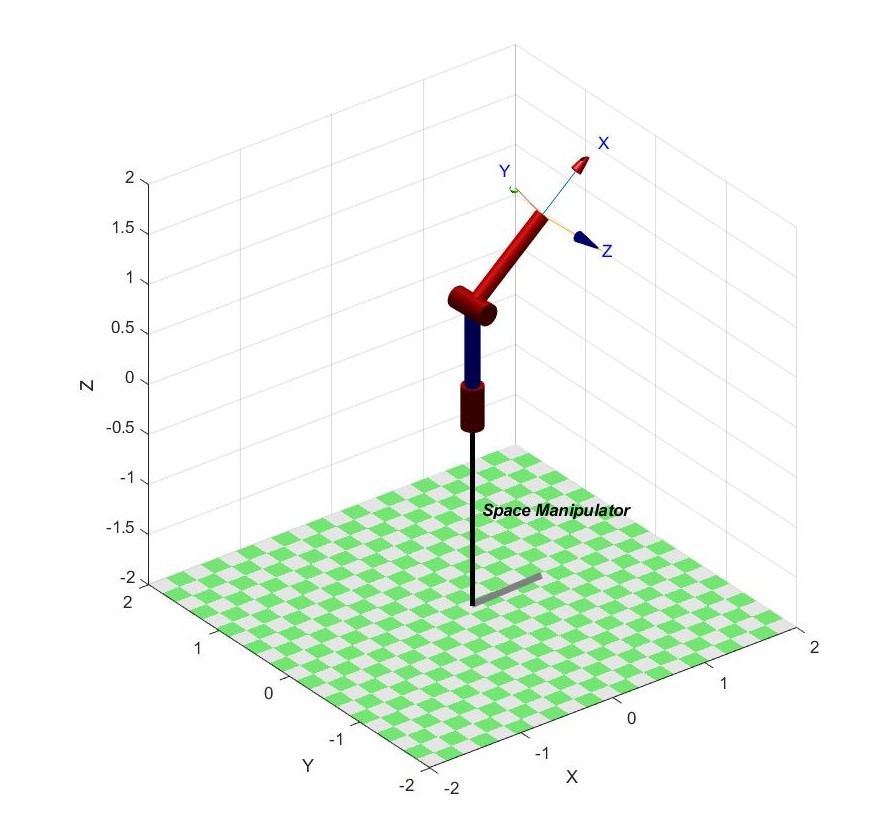
\includegraphics[width=0.6\textwidth]{figures/Manipulator_ritagliata.jpg}
        \caption{Manipulator design.}
        \label{fig:manipulator}
\end{figure}

Considering the spacecraft’s central body like a cube of side length L = 1 m. The two important reference frames we consider are:
\begin{itemize}
\item The \textbf{LVLH frame (Local Vertical Local Horizontal)}, located at the cube’s center with the z-axis pointing towards the planet, the y axis parallel to the spacecraft velocity and the x-axis to get a right-handed triad. 
\item \textbf{The manipulator base frame}, located on the side of the spacecraft where the y-axis of the LVLH heads. 
\end{itemize}


The transformation from the LVLH frame and base frame is defined as the sequence of rotation around y axis by $\pi/2$, rotation around z axis by $\pi/4$ and translation by $L/2$ along the z-axis, as can be seen in the equation \ref{eq: T_lvlh_b}.\

The rotation of 45 deg around the z axis is to adjust and orient the manipulator's workspace in order to permit a better pointing of Mars and Earth both and contemporary to guarantee that the joint angles do not get too close to the limits of the workspace avoiding singularities.
\begin{equation}
  ^{B}_{LVLH}T = R_{y}\left(\dfrac{\pi}{2}\right) R_{z}\left(\dfrac{\pi}{4}\right) D_{z}\left(\dfrac{L}{2}\right)  
  \label{eq: T_lvlh_b}
\end{equation}

The figure XXX shows the s/c with the LVLH and Base frames attached on it.



\subsection{Jacobian matrix}
Forward kinematics allows to know the \textit{end-effector} (EE) position $p_{EE}(q)$ as a function of the joint variables. In addition to it, is possible to express the linear and angular components of the end effector's velocity by means of the geometric Jacobian ~\protect{\cite{robotics_reference}}. \\In the 2-Link manipulator case, the Jacobian is a $6\times{2}$ matrix, composed by the linear and angular Jacobian, $J_L$ and $J_A$ respectively, such that 
$J = \begin{bmatrix}
J_L\\
J_A\\
\end{bmatrix}$, and:

\begin{equation}
    \centering
    \left\{\begin{split} 
      \dot{p}_E &= J_L(q)\,\dot{q}  \\
      \omega_E &= J_A(q)\,\dot{q}
      \end{split}\right.
\end{equation}
\break
By doing so, it is possible to express a direct relation between the joint and EE velocities based only on geometric quantities. \\Dealing with two revolut joints, each of them is expressed by the following Jacobian:
\begin{equation}
    \centering
    \left\{\begin{split} 
    %J_L(q) =  z_{i-1}\times{p_{i-1,E}} = \pdv{p_{0,E}(q)}{q_i} \\
     J_{L_i}(q) &=  z_{i-1}\times{p_{i-1,E}} = \dfrac{\partial{p_{0,E}(q)}}{\partial{q_i}} \\
     J_{A_i}(q) &= z_{i-1}
     \end{split}\right.
\end{equation}
where $z_{i-1}$ and $p_{i-1,E}$ are both referred to the base frame of the manipulator, $i \in \{1,2\}$.\\

%\textcolor{red}{Informazioni prese da dispense Adriano e libro di sicialiano, oriolo etc..."}

%\textcolor{blue}{$J*atm_drag$ serve slide 28 jacobian: per realazionare con joint space}



\subsection{Dynamical equations}
The dynamical model is computed via the Lagrangian method; so the kinematic energy is computed for each link as follows:
$$T_i = \frac{1}{2}\,m_i\,v_{C,i}^T\,v_{C,i} + \frac{1}{2}\,^{i}\omega_i^{T}\,I_i\,^{C_i}I\,^{i}\omega_{i}$$
then, \underline{under the hypothesis of null potential energy in space ($u=0$)}, the torques are obtained through the kinematic energy:
$$\dfrac{d}{dt}\dfrac{\partial{T(\Theta,\dot{\Theta})}}{\partial{\dot{\Theta}}}-\dfrac{\partial{T(\dot{\Theta},\Theta)}}{\partial{\Theta}}=\tau$$
being: 
$\Theta = \begin{bmatrix} \theta_1;\theta_2\end{bmatrix}^{T}$.\\

To retrieve the Mass matrix, $M$, it is possible to extract the individual terms by deriving the total kinematic energy two times with respect to $\dot{\Theta}$, remembering that these are the coefficients multiplying the velocities of the joints.\\

The Velocity matrix, $V$, is retrieved through the use of the Christoffel Matrices, $C_i$. Thus, being $m_{i,j}$ the Mass matrix' coefficients and $c_{ij}$ the Christoffel symbols referred to the $k$ joint, with:
$$c_{ji}^k=c_{ij}^k=\frac{1}{2}\,\left(\dfrac{\partial{m_{kj}}}{\partial{q_i}}+\dfrac{\partial{m_{ki}}}{\partial{q_j}}-\dfrac{\partial{m_{ij}}}{\partial{q_k}}\right)$$
and finally:
$$V_k = \dot{\Theta}^{T}\,C_k\,\dot{\Theta}$$

From this formulation it is also possible to split the Velocity matrix to take in account the Coriolis and centrifugal coefficients with the $B(\Theta)$ and $C(\Theta)$ matrices respectively; in this way the Configuration-Space equation cam be written as:
$$M(\Theta)\,\ddot{\Theta}+B(\Theta)\,[\dot{\Theta}\dot{\Theta}]+C(\Theta)\,[\dot{\Theta}]^2=\tau$$
\\
\textcolor{red}{CAPIRE MEGLIO COME INSERIRE I TERMINI DI FRIZIONE}

\subsection{Trajectory planning}

After having obtained the orbits' configuration from the first task, we know the positions of Mars and Earth in a certain time window, and expressed in the LVLH frame. Then, as regards the mars target, we point at the off-nadir angle of the planet, rather than the nadir angle itself. Thus we have shifted the target by rotating the LVLH frame of 15 degrees, along an arbitrary axis. In our case, this last was the y-axis.\\
Now, it's possible to generate the robot trajectory that points at the targets correctly, by satisfying any of the constraints imposed by the task guidelines. Specifically, the approach we followed is the \textbf{indirect trajectory planning in the Joint Space}, which comprehends three main steps:
\begin{enumerate}
    \item \textbf{Inverse kinematics}: Given any initial configuration $q_i \in \mathbb{R}^2$, the final configuration $q_f \in \mathbb{R}^2$ is computed according to the solution of the inverse kinematics problem.
    \item \textbf{Path planning}: The path $q(s)$ between $q(s_i) = q_i$ and $q(s_f) = q_f$ is determined through quintic polynomials for the joint configurations, velocities and accelerations, parameterized by a timing law ($s=t/T$).
    \item \textbf{Timing law computation}: The trajectory is completed by the resolution, of the timing law, which is computed by taking into account the additional constraints on the motor torques, if violated the total execution time to execute the trajectory will be incremented.
    
\end{enumerate}

\subsubsection{Inverse Kinematics}
The inverse kinematics problem has been presented as a rather difficult task to resolve, due to the fact that our manipulator has 2 degrees of freedom, while the orientation of the end effector (EE) is SO(3), thus requires 3 degrees of freedom, making both classic analytic and numerical methods not effective.\\
Consequently, we had to develop a rather unconventional method to solve the inverse kinematic problem. Specifically, for each pointing direction the corresponding joint configuration is obtained as the solution of a constrained non-linear optimization problem, which aims to find the joint angles $q^*$ such that the EE, the tip of the antenna and the considered planet are all lying on the same line.\\
Before formulating the problem, it is necessary to define some notations.\\
Let $^Fp_{EE}(q)$ be the EE position, expressed by the joint angles, in a generic reference frame $F$, and $^Fp_{tip}(q)$ the antenna position evaluated in the same manner. Then let us consider the target $^Ft$, as the planet's position for which we are interested in for the pointing, and $Q_{max}, Q_{min}$ as the joint bounds that must be satisfied in the solution. ($Q_{max}, Q_{min} \in \mathbb{R}^2$).\\ Finally we refer to $V_{EE}(q) = ^Ft - ^Fp_{EE}(q)$, and $V_{tip}(q) =  ^Ft - ^Fp_{tip}(q) $ as the distance between the EE and the target, and the antenna with the target respectively.\\
The optimization task can be formulated as follows.\\

\begin{subequations}
\label{eq:optim}
\begin{align}
    \underset{X}{\text{minimize}}
        & \quad ||V_{EE}(q) \times V_{tip}(q)||_2^2 \label{eq:objective}\\
    \text{subject to} 
        & \quad -V_{tip}(q)\cdot V_{EE}(q) \leq 0 \label{eq:scalar}\\
        & \quad \quad q_i \leq Q_{i,max} \quad i = 1, 2 \nonumber\\
        & \quad -q_i \leq Q_{i,min} \quad i = 1, 2 \nonumber
\end{align}
\end{subequations}

In Equation \ref{eq:objective}, the global solution of the problem would involve that the two lines are parallel, and it is only possible by zeroing the cross product. Additionally we do not want to have the EE as the middle point between the target and the antenna position, such scenario can be avoided by imposing the constraint in Equation \ref{eq:scalar}.
In our experiments, the reference frame $F$ chosen was LVLH.\\
The solution is obtained through \textit{fmincon}{} solutor from the \textit{Matlab Optimization Toolbox} ~\protect{\cite{Optimization_Toolbox}}.


\subsubsection{Path planning}
All sequential configurations determined as solution to the inverse kinematic problem have been interpolated through a chain of fifth order polynomials, in order to be able to compute a continuous path up to the second order derivative (acceleration). The degree of the polynomial is essential, due to the fact that the manipulator is controlled in torque, therefore the commands for each time-step should be deployed in acceleration in order to be used by the controller. \\

Regarding the formulation, the quintic polynomial and its derivatives are used to define each path segment in position, velocity and acceleration as follow:
\begin{align*}
\theta(s)&=a_0\,+a_1\,s+a_2\,s^2+a_3\,s^3+a_4\,s^4+a_5\,s^5\\
\dot\theta(s)&=a_1\,+2\,a_2\,s+3\,a_3\,s^2+4\,a_4\,s^3+5\,a_5\,s^4\\
\ddot\theta(s)&=2\,a_2+6\,a_3\,s+12\,a_4\,s^2+20\,a_5\,s^3
\end{align*}
where $s=s(t)=\dfrac{t}{T}\in{[0,1]}$ is the timing law associated to the path segment (this allows to compute T in a second movement, in order to be able to elongate the the time, in order to decrease the acceleration, in case 
 during path the boundaries on the torqure are violated). \\
Then, in order to determine the coefficients the following boundary conditions on position velocity and acceleration are imposed:
\begin{align*}
\theta_i(t_0)&=\theta_{i,0} \;\;\;\;\;\; ; \;\;\;\;\;\ \dot{\theta}_i(t_0)=\dot{\theta}_i(t_f)=0 \\
\theta_i(t_f)&=\theta_{i,f}  \;\;\;\;\;\; ; \;\;\;\;\;\; \ddot{\theta}_i(t_0)=\ddot{\theta}_i(t_f)=0 
\end{align*}

where $\theta_{i,0}$ and $\theta_{i,f}$ are respectively the initial and final configuration of the segments, while $t_0$ and $t_f$ are the initial final time steps.
Finally, by computing the Jacobian a linear system is obtained, so the desired evolution in time of the joint angles, velocity and accelerations is easily computed.\\

\subsubsection{Timing law computation}
Once the path has been computed, a timing law has to be formulated in order to guarantee that the torque required at each step does not exceed the boundaries imposed by the motors. The first attempt is done imposing $T=1\; s$ in the path from the previous step and compute the torque erogated by the motor ("\textit{motor side}") as follows:
$$\tau_m=\left (I_m+\dfrac{I}{\eta^2}\right)\ddot{\theta}_m + \left(b_m+\dfrac{b}{\eta}^2\right)\,\dot{\theta}_m + \dfrac{\tau_c}{\eta}$$
where: $\eta$ is the gear ratio, $b_m$ is the viscous friction coefficient, $\tau_c$ the static friction and $I$ and $I_m$ the inertia of the motor and the joints respectively. \\
Then, if the torque exceed the boundaries, a time scaling factor is computed as:
$$\lambda = \sqrt{max_i\bigg\{\frac{\hat{\tau}_{i,max}}{\tau_{i,max}}\bigg\}}$$
where $\hat{\tau}_{i,max}$ id the highest value of the torque erogated by the i-th joint motor, while $\tau_{i,max}$ is the corresponding boundary. The idea is simply to compute $\lambda < 0$ depending on the "most violated" constraint and then scale time as: $T'=\lambda\;T$



\subsection{Controller}
\subsubsection{External disturbance}
At this point the trajectory is available in discrete time, for each time step we can retrieve the configuration through the dynamic model. Now, it is possible to take in account the atmospheric drag, $a_D$, modelled as follows:
$$a_D=\frac{1}{2}\,c_D\,\rho\,S_A\,v_{SC}^2$$
where:
\begin{itemize}
    \item $c_D = 0.3$, is the drag coefficient;
    \item $\rho = 10^{-14}\; [kg/m^3]$, is the atmospheric density of Mars atmosphere considered constant;
    \item $S_A = 28.27\; [m^2]$, is the surface of the antenna, supposed to be always fully exposed;
    \item $v_{SC}$, is the spacecraft velocity.
\end{itemize}
To relate this external disturbance to the joint space is sufficient to multiply by the transposed of the Jacobian. Under the hypothesis that the drag effects are only dependent on the position of the EE, it is possible to write:
$$\tau_a=J_L^T\,a_D$$

\subsubsection{Mismodelling}
With the aim of dealing with a closer to reality model, a mismodeling is introduced. So, the "true" variables are created by the sum of the nominal value and the term given by the multiplication of an arbitrary tolerance and the AWGN. For a general variable X we have:
$$\hat X = X_{nom} + AWGN*X_{toll} $$
where $X_{nom}$ is the nominal value of the variable and the $X_{toll}$ is the arbitrary tolerance we attributed to the same variable, as the Table \ref{tab:TAB} (to be noticed, tolerances have been chosen to be three order smaller than the nominal value).

\begin{table}[!h]
\begin{center}
\begin{tabular}{||c c c||} 
     \hline
    \multicolumn{3}{|c|}{Tolerances List} \\
    \hline
    Variables Name& Tolerance &Measurement unit\\
    \hline
     Link Length & $10^{-3}$ & m\\
     Link Radius & $10^{-4}$ & m\\
     Link Thickness & $10^{-6}$ & m\\
    \hline
\end{tabular}
\caption{\label{tab:TAB} Tolerance measures.}
\end{center}
\end{table}

These mismodelling will have an impact on the computed of the "true" dynamic matrices, which will be used to compute the "true" dynamic model. This is important for the sake of the simulations, due to the fact that the need of a controller is actually driven by the mismodeling itself and its effects on the execution of the trajectory.


\subsubsection{Control scheme}
The controller is modelled as a feedforward nonlinear control with external perturbations (provided by the simulated atmospheric drag).\\

The control law can be written as:
$$ \tau = \tau'\;M(q) + V(\theta,\dot\theta)+F(\theta,\dot\theta)-\tau_a$$
where:
\begin{itemize}
    \item {$\tau'=\ddot{\theta}_d+k_v\,\dot{e}+k_p\,e$ is the command in acceleration, with:
        \subitem { -   $k_v=400$ and $k_d=2\,\sqrt{k_v}$ being the control gains.}
        \subitem { -   $e=\theta_d-\theta$ is the error in joint position}
        \subitem { -   $\dot{e}=\dot{\theta_d}-\dot{\theta}$ is the error in joint velocity.}}
    \item{$M(q)$ is the nominal inertia matrix.}
    \item{$V(\theta,\dot\theta)$ is the nominal Coriolis and centrifugal term.}
    \item{$F(\theta,\dot\theta) = \tau_c $ is the value of the friction, computed with a fixed value depending on the sign of the joint velocity}
    \item{$\tau_a$ is the drag effect.}
    
\end{itemize}

\begin{figure}[htp]
    \includegraphics[width=\textwidth]{figures/control_scheme.jpeg}
    \caption{Control scheme used for the robot model.}
\label{fig:ConSch}
\end{figure}

Proceeding with the code implementation, the controller receives in input the desired trajectory and the previous errors ($e,\dot e$) and then follows the next steps:\\
\begin{enumerate}
    \item {Get the real joint configuration and velocity from the desired configuration and the previous error.}
    \item Get the nominal dynamic terms ($M,V,\tau_c,\tau_a$).
    \item Compute the command in acceleration considering the nominal dynamics.
    \item Compute the true dynamic terms ($\hat M,\hat V,\hat \tau_c,\hat \tau_a$)
    \item Get the error in acceleration considering the following equation:
    $$\ddot{e}=\ddot{\theta}_d- \hat M^{-1} (-V+\tau_c+\tau_a+\tau)$$
    \item Integrate the errors in velocity and acceleration, with \textit{Ode113} (where we chose both relative and absolute tolerance at $10^{-4}$) to get the final value of the error ($e,\dot e$).
\end{enumerate}
Finally, after the integration the integral error is retrieved and the effective trajectory can be evaluated.\\


\subsection{Experiment setup and results}
%description of the setup of the orbits data and stuff
%plots of the trajectory execution 

\bibliographystyle{abbrv}
\bibliography{ref}

\end{document}  